\section{Finger names}

When playing guitar, your fingers will be given a name. This makes it easier in music notation to indicate which finger should be used. The names are shown in \ref{fig:finger_names}.

\begin{figure}[h]
    \centering
    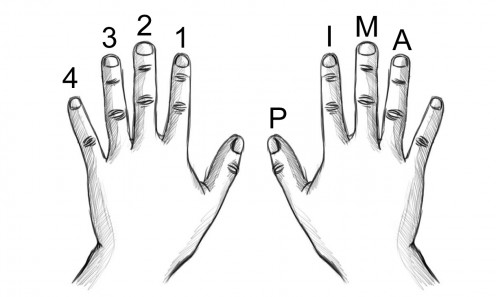
\includegraphics[width=0.7\textwidth]{../../Images/guitar-finger-tips_pima.jpg}
    \caption{Names of the fingers \cite{FingerNames}}
    \label{fig:finger_names}
\end{figure}

\subsection{Free and rest stroke}

With a free stroke you hold your right hand in a relaxed position over the strings (see \ref{fig:free_stoke_hand_position}). To play a string, move your finger through the string without lifting the upper part of your finger. Your finger should slightly curl into your hand. Once you made the sound, move your finger back to the relaxed position.

The trick now is, to not hit the other strings, and to not 'pluck' the string (making a buzzing sound).

% TODO: Change picture to ukulele

\begin{figure}[h]
  \begin{subfigure}[b]{0.45\textwidth}
    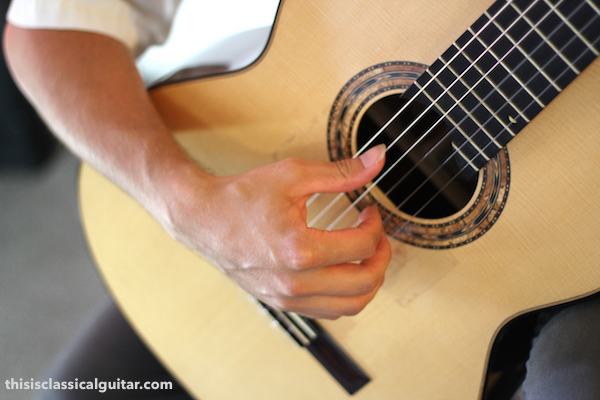
\includegraphics[width=\textwidth]{../../Images/Bradford-right-hand-close-2016.jpg}
    \caption{}
    \label{fig:}
  \end{subfigure}
  \hfill
  \begin{subfigure}[b]{0.45\textwidth}
    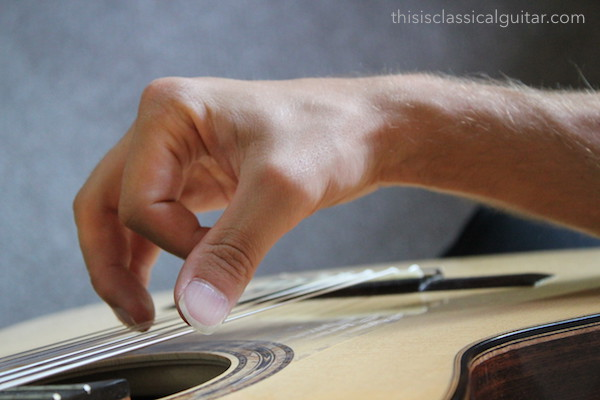
\includegraphics[width=\textwidth]{../../Images/brad-right-stroke-2016.jpg}
    \caption{}
    \label{fig:}
  \end{subfigure}
  \caption{Free stroke position \cite{FreeStrokePositionBradlyWerner}}
  \label{fig:free_stoke_hand_position}
\end{figure}

A rest stroke may sound a bit louder (but with some practicing a free stroke can be as loud). Like the name suggests, a rest stroke means that you move your finger through a string to play it, but now you let your finger rest on the next string.

\newpage

\subsection{Exercises}

In the exercises below you see some symbols above the notes. The numbers with circles around them indicate on which string the note should be played (this can also be seen from the TAB). The \textit{i} and \textit{m} indicate which right-hand finger should be used to play the note.

Play exercise \ref{fig:ukulele_exercise_rest_free_stroke} first with a rest stroke and then with a free stroke to feel the difference.

\begin{figure}[h]
    \centering
    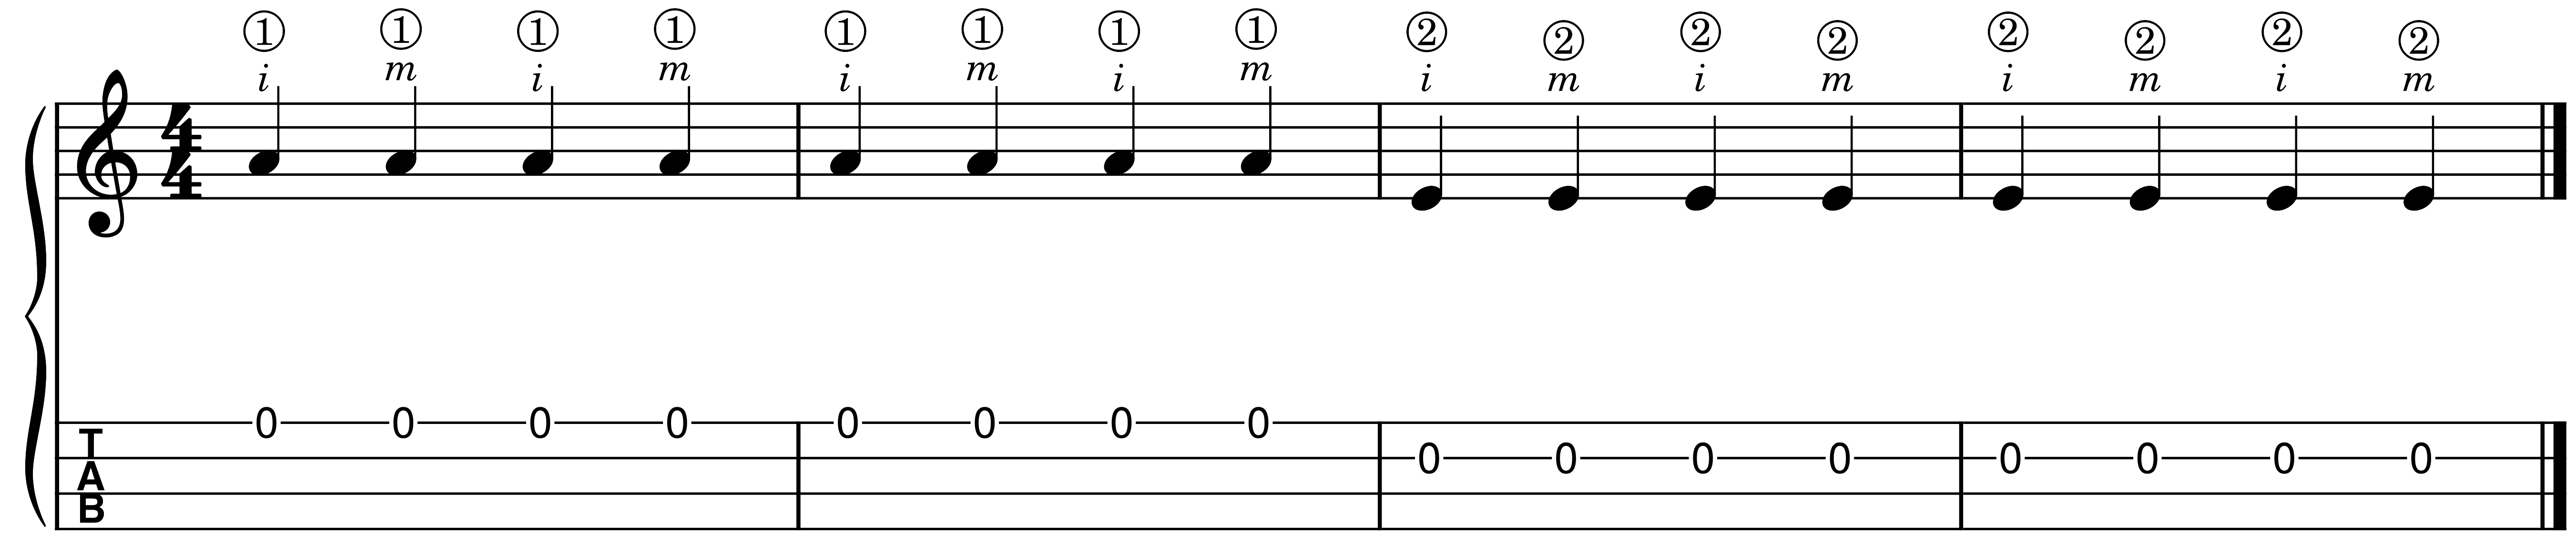
\includegraphics[width=\textwidth]{../../MuseScore/Ukulele/UkuleleExerciseFreeAndRestStokeSimple.png}
    \caption{Exercise: rest and free strokes}
    \label{fig:ukulele_exercise_rest_free_stroke}
\end{figure}

This second exercise (\ref{fig:ukulele_exercise_i_m_string_change}) is similar to \ref{fig:ukulele_exercise_rest_free_stroke}, but a bit more challenging.

\begin{figure}[h]
    \centering
    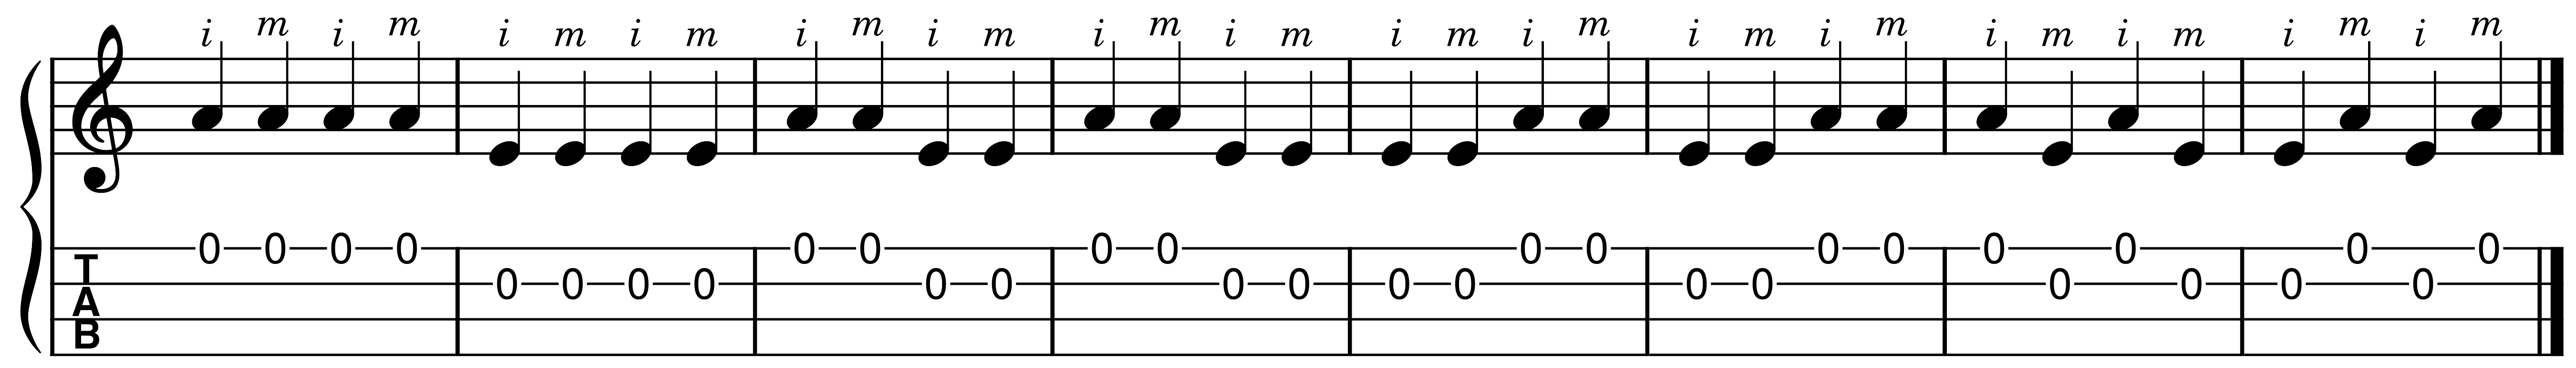
\includegraphics[width=\textwidth]{../../MuseScore/Ukulele/UkuleleExerciseFreeAndRestStokeStepTwo.png}
    \caption{Exercise: changing strings with \textit{i} and \textit{m} fingers}
    \label{fig:ukulele_exercise_i_m_string_change}
\end{figure}

\newpage

In \ref{fig:ukulele_exercise_fretting_fingering_first_string} you will also use your left hand. The numbers above the notes indicates which left-hand finger should be used to press the fret. Play this exercise using alternating \textit{i} and \textit{m} fingers. 

\begin{figure}[h]
    \centering
    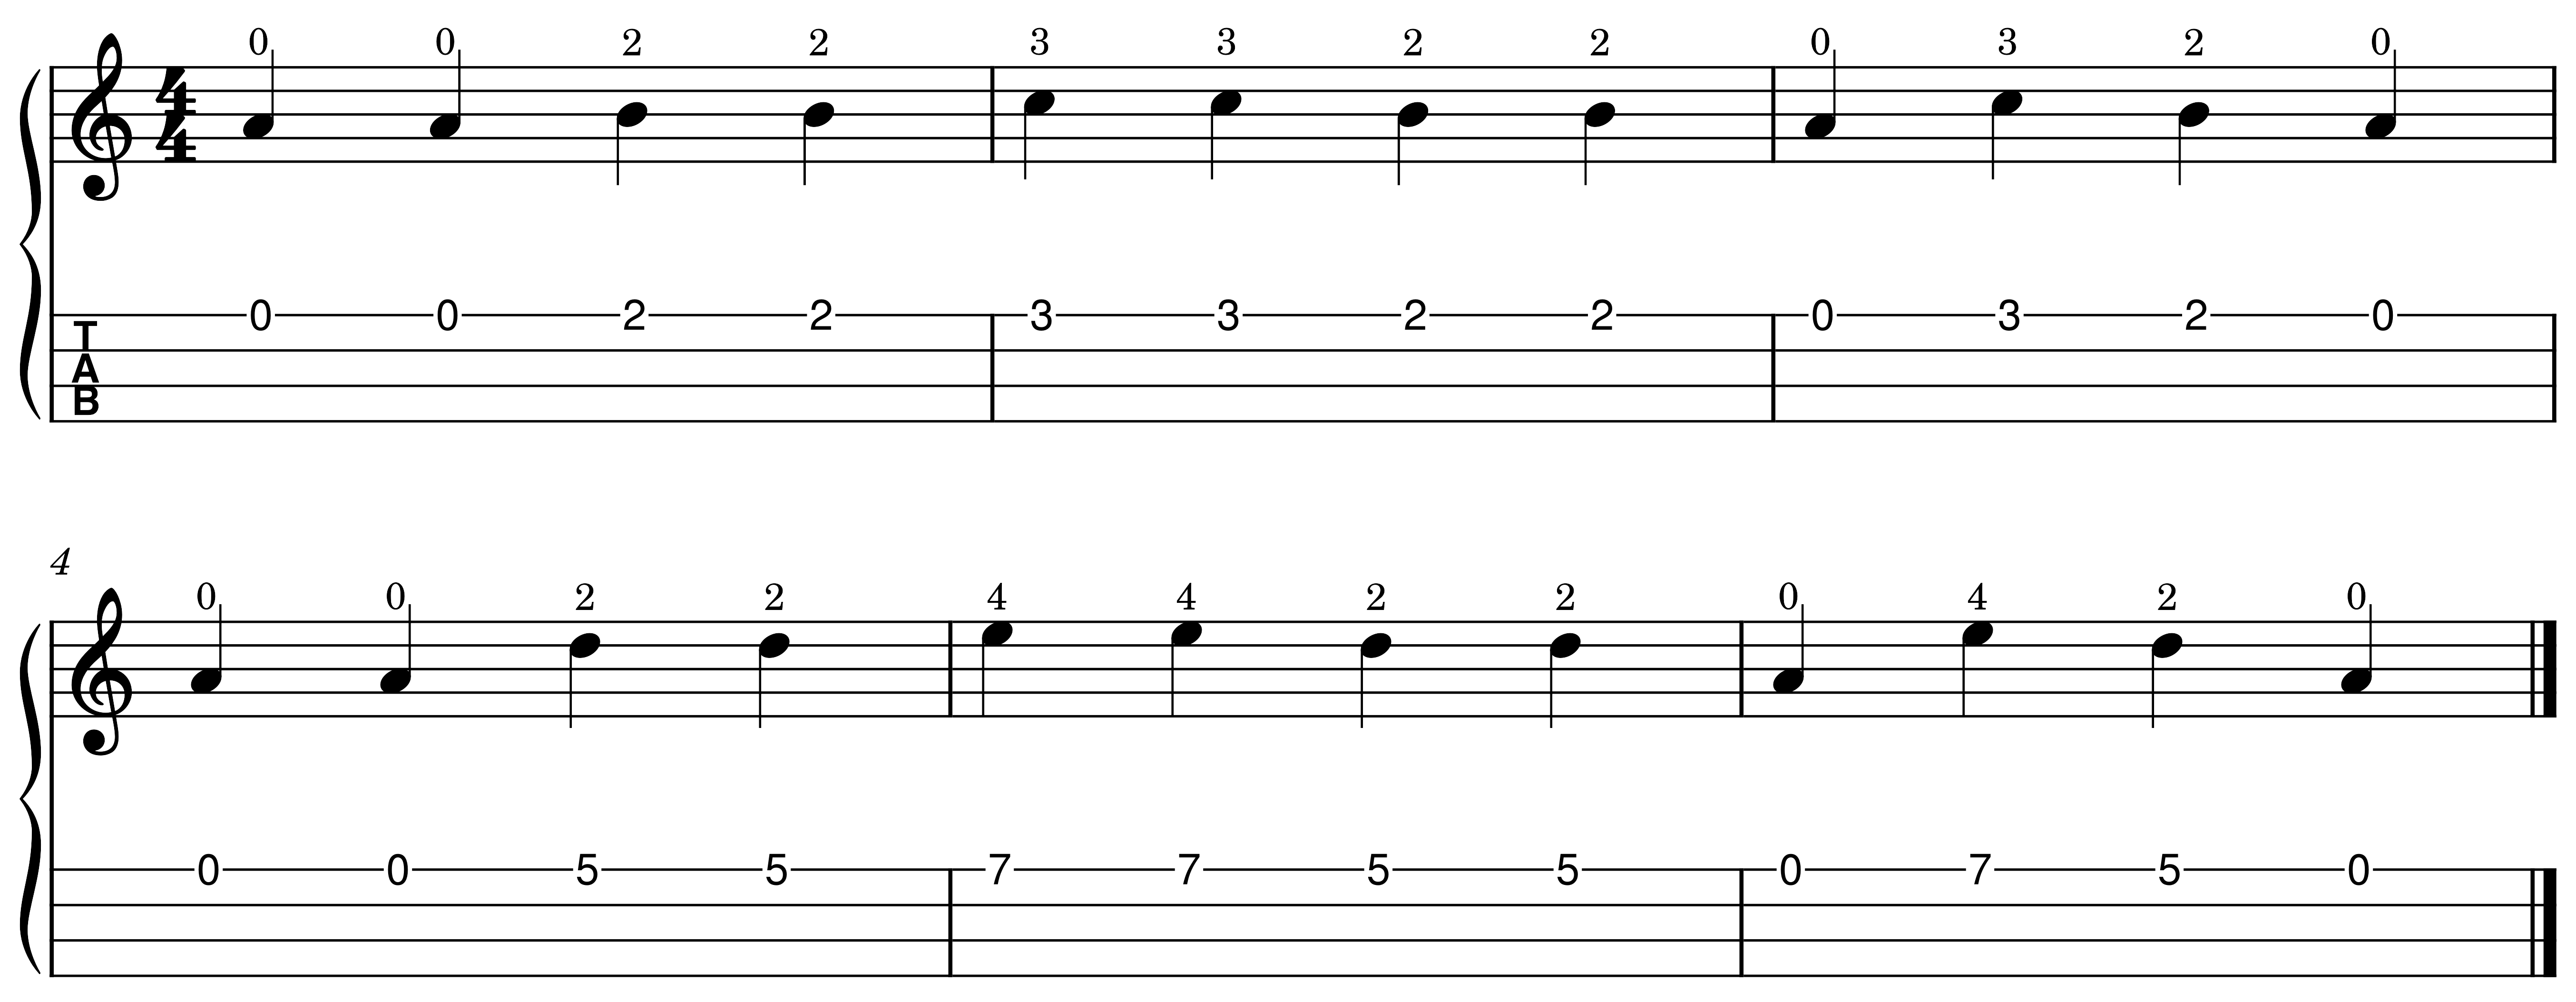
\includegraphics[width=\textwidth]{../../MuseScore/Ukulele/UkuleleExerciseFirstStringFretting.png}
    \caption{Exercise: fretting on 1st string}
    \label{fig:ukulele_exercise_fretting_fingering_first_string}
\end{figure}

Exercise \ref{fig:ukulele_exercise_fretting_fingering_first_and_second_string} is adds another string to the exercise.

\begin{figure}[h]
	\centering
	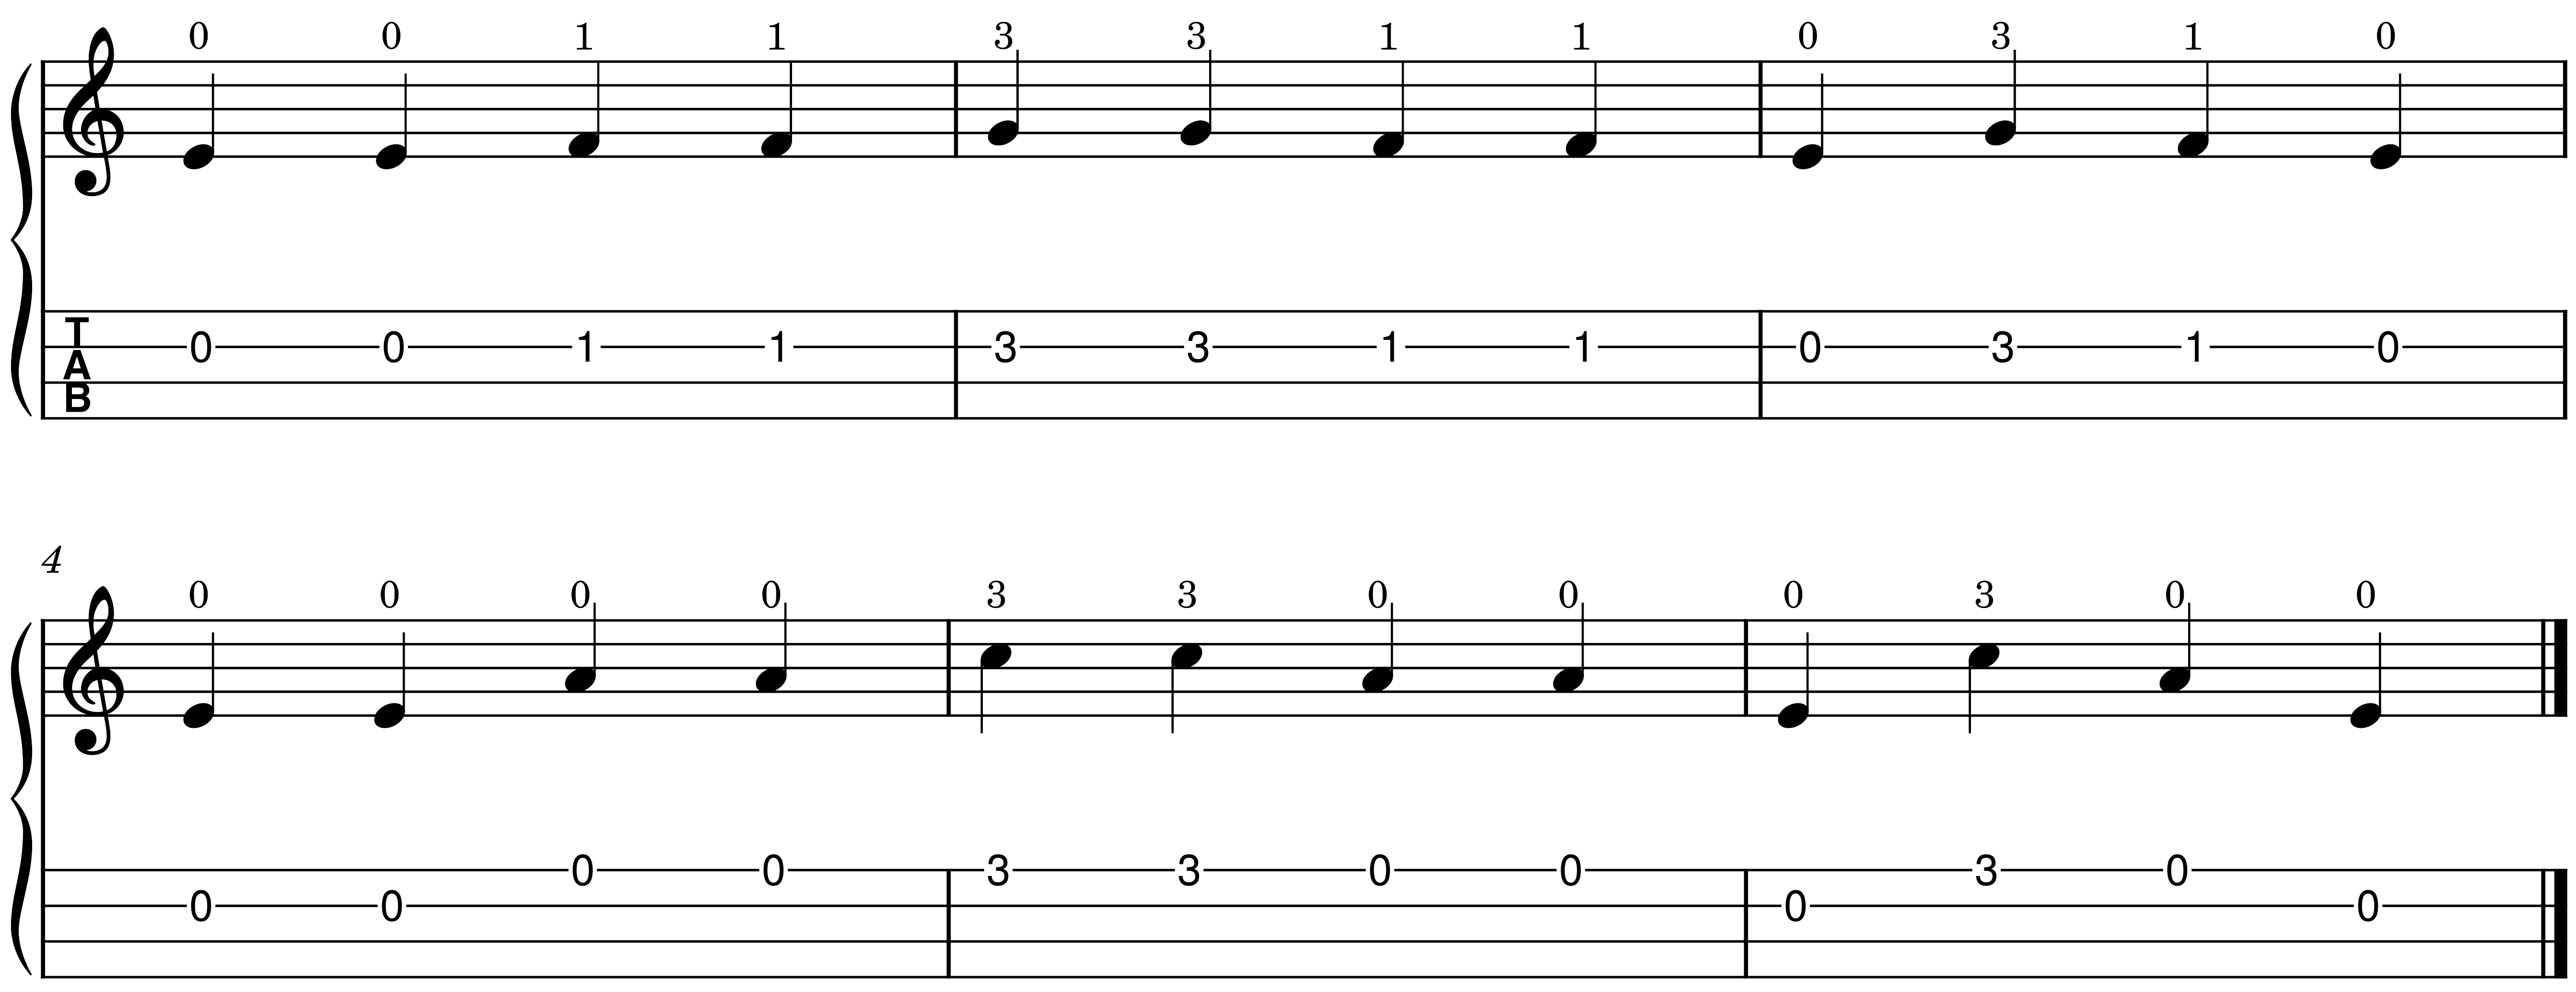
\includegraphics[width=\textwidth]{../../MuseScore/Ukulele/UkuleleExerciseTwoStringFretting.png}
	\caption{Exercise: fretting on 1st and 2nd string}
	\label{fig:ukulele_exercise_fretting_fingering_first_and_second_string}
\end{figure}